\documentclass{beamer}
\usetheme{Madrid}
\AtBeginSection[]{
  \begin{frame}
  \vfill
  \centering
  \begin{beamercolorbox}[sep=8pt,center,shadow=true,rounded=true]{title}
    \usebeamerfont{title}\insertsectionhead\par%
  \end{beamercolorbox}
  \vfill
  \end{frame}
}

\AtBeginSubsection[]{
  \begin{frame}
  \vfill
  \centering
  \begin{beamercolorbox}[sep=8pt,center,shadow=true,rounded=true]{title}
    \usebeamerfont{title}\insertsubsectionhead\par%
  \end{beamercolorbox}
  \vfill
  \end{frame}
}



\usepackage{subcaption}
\usepackage{tikz}
\usetikzlibrary{positioning} 
\usetikzlibrary{matrix}
\usetikzlibrary{calc}
\newcommand{\z}{\mathbf{z}}
\newcommand{\uout}{u_{out}}
\newcommand{\vout}{v_{out}}
\newcommand{\uoutdum}{u_{out}^{dum}}
\newcommand{\uinplus}{u_{in}^{+}}
\newcommand{\uinminus}{u_{in}^{-}}
\newcommand{\winl}{w_{in}^{l}}
\newcommand{\win}{w_{in}}
\newcommand{\uin}{w_{in}}
\newcommand{\vin}{v_{in}}

\DeclareMathOperator*{\plusrightarrow}{\ensuremath{\xrightarrow{+}}}
\DeclareMathOperator*{\minusrightarrow}{\ensuremath{\xrightarrow{-}}}
\DeclareMathOperator*{\plusleftarrow}{\ensuremath{\xleftarrow{+}}}
\DeclareMathOperator*{\minusleftarrow}{\ensuremath{\xleftarrow{-}}}
\usetikzlibrary{shadows,positioning}
\colorlet{colD}{red!40}
\colorlet{colIP}{cyan!40}
\colorlet{colV}{blue!40}
\colorlet{colBorder}{gray!70}


\title[SLIDE]{MLDB Presentation\\SLIDE: Sub-LInear Deep Learning Engine}

\author[Beidi Chen et al.]{Beidi Chen \and Tharun Medini \and James Farwell \and Sameh Gobriel \and Charlie Tai \and Anshumali Shrivastava}
\date{\today}

\begin{document}
\begin{frame}
    \titlepage
\end{frame}

\begin{frame}
    \frametitle{Overview}
    \tableofcontents
\end{frame}


\section{Motivation}
\begin{frame}
    \frametitle{Era of Deep Learning}
    \begin{figure}[ht!]
        \centering
        \begin{subfigure}{0.4\textwidth}
            \centering
            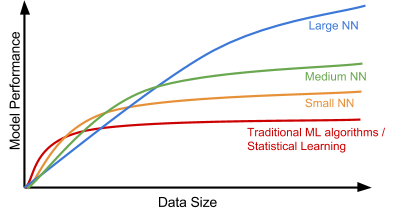
\includegraphics[width=1.2\textwidth]{images/deep learning.png}
            \caption{Model Performance wrt Dataset size}
            \label{fig:deep-learning}
        \end{subfigure}
        \begin{subfigure}{0.4\textwidth}
            \centering
            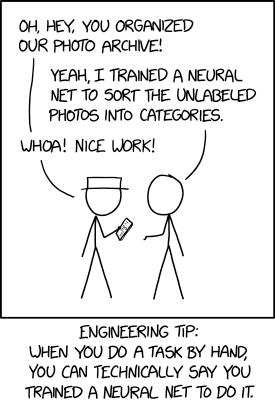
\includegraphics[width=0.7\textwidth]{images/xkcd.png}
            \caption{Fun xkcd comic}
            \label{fig:deep-learning}
        \end{subfigure}

    \end{figure}
    
\end{frame}
\begin{frame}
    \frametitle{Trends}
    \begin{itemize}
        \item Large datasets $\rightarrow$ More Data
        \item Big models (Eg, 17B parameter NLP models)
        \item Improvements in optimizations and gradient descent
        \item \structure{Matrix multiplication} is a computational bottleneck
        \item Many approaches exists such as \structure{GPUs}
    \end{itemize}

\end{frame}

\subsection{Existing Approaches}
\begin{frame}
    \frametitle{Low Rank structure}

    \begin{minipage}{0.6\textwidth}
        \begin{itemize}
            \item $W \in \mathbb{R}^{m\times n}$ is weight matrix
            \item $W$ has a low-rank structure $W=UV$
            \item $U\in \mathbb{R}^{m\times r}$ and $V\in \mathbb{R}^{r\times n}$, where $r \ll \min(m,n)$
            \item Equivalent representation with $I$ activation function is better
            \item $\mathcal{O}(mn)$ becomes $\mathcal{O}(mr+rn)$
            \item \structure{Better storage} of parameters as well
            \item But still needs dense gradient update, cannot parallelise asynchronously
        \end{itemize}
    \end{minipage}\hfill
    \begin{minipage}{0.4\textwidth}
        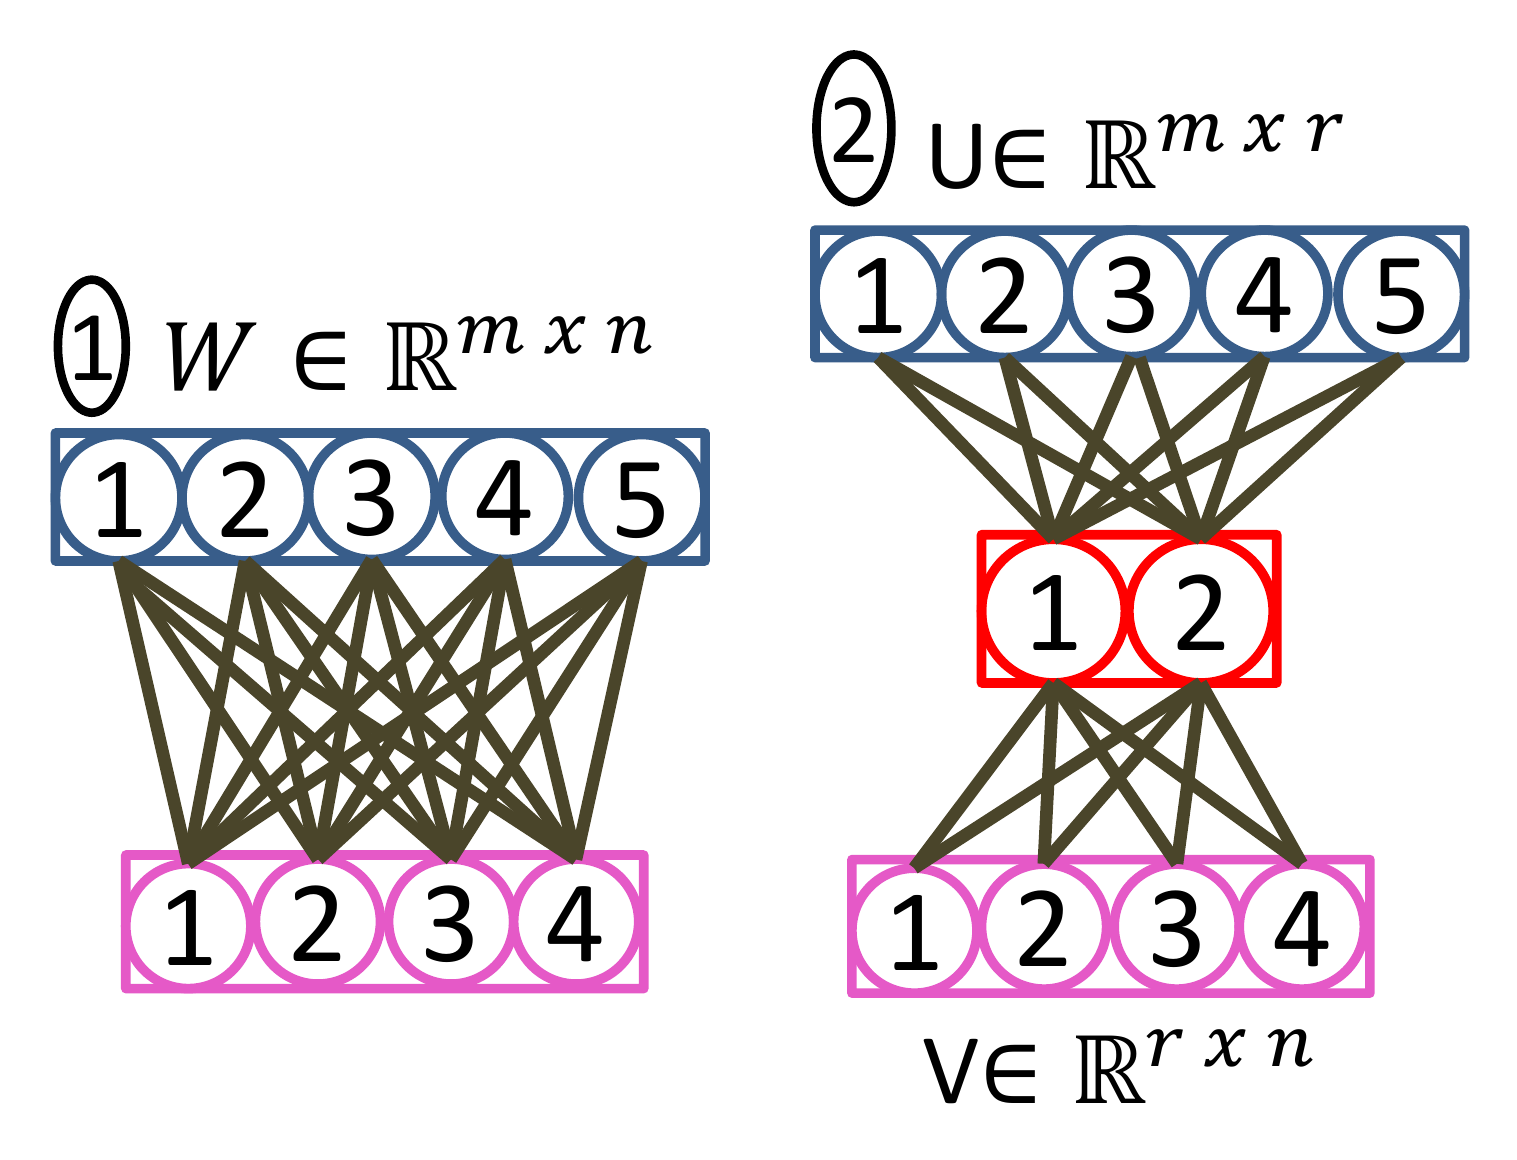
\includegraphics[width=\textwidth]{images/Low_Rank.png}
    \end{minipage}

\end{frame}

\begin{frame}
    \frametitle{Dropout and Sparsity}
    \begin{minipage}{0.5\textwidth}
        \begin{itemize}
            \item Well known regularization method for Neural Networks
            \item With probability $p$ neurons in each layer is \structure{turned off}
            \item Used during training to ensure model generalizes 
            \item Sparsity above 50\% tends to begin hurting performance
        \end{itemize}
    \end{minipage}\hfill
    \begin{minipage}{0.5\textwidth}
        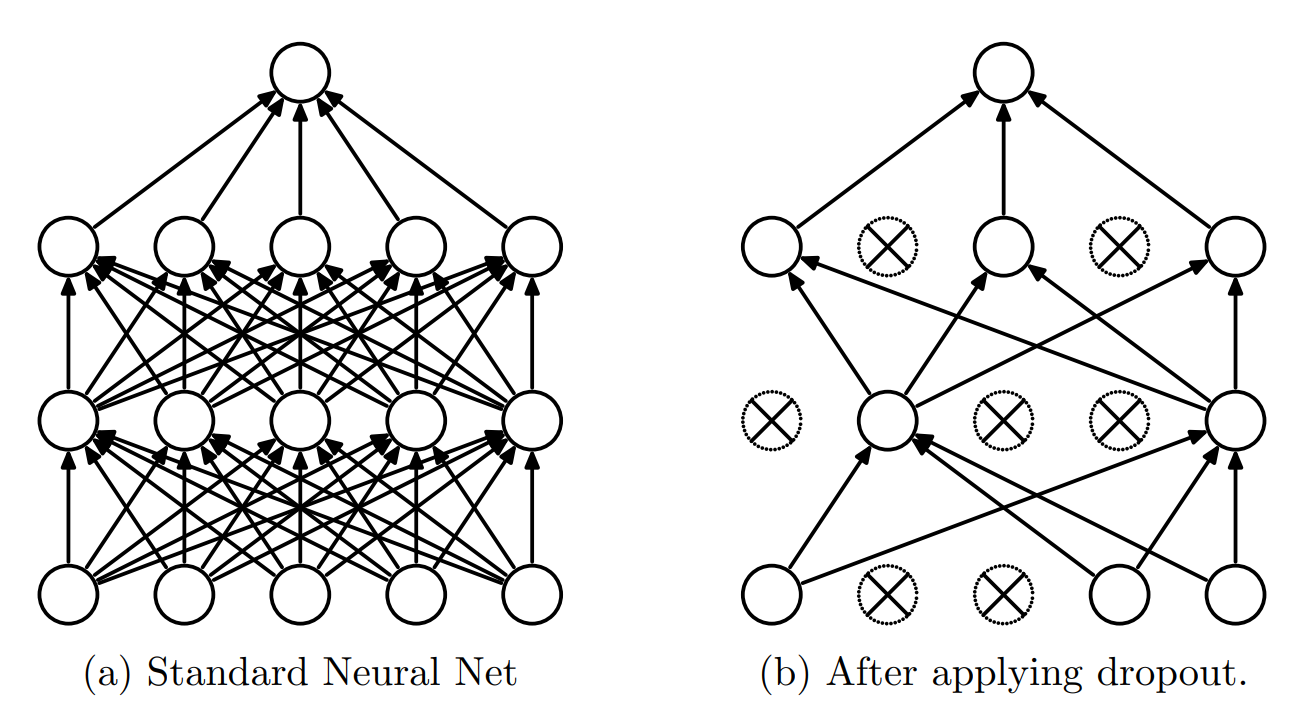
\includegraphics[width=\textwidth]{images/dropout.png}
    \end{minipage}
    
\end{frame}

\begin{frame}
    \frametitle{Adaptive Dropout}
    \begin{itemize}
        \item $p$ is \structure{chosen adaptively} based on activation of neurons in a layer
        \item And perform forward and backward propagation only on the \structure{active neurons} in each layer
        \item Reduces the number of neurons to compute in each layer
        \item RELU is sparse in nature and filters negative activations
        \item \cite{Lei_adaptive_dropout} use a Bernoulli distribution proportional to activation of each neuron
        \item Still requires computing \structure{all activations} to identify active neurons
    \end{itemize}
    

\end{frame}
\subsection{Problem Setting}
\begin{frame}
    \frametitle{Sampling Problem}
    \begin{itemize}
        \item Each layer has $N$ time-varying sampling weights
        \item Weights a function of activations of neurons, $w_{1}^{t},w_{2}^{t},\dots,w_{N}^{t}$
        \item At each time $t$, we need to sample $x_i$ with probability $w_{i}^{t}$
        \item Sampling cost is $\mathcal{O}(N)$ for each time step $t$
    \end{itemize}
    \begin{block}<1>{Problem}<2>
        Can we efficiently sample the neurons in a layer to find the \structure<2>{active neurons} given the input to the layer?
    \end{block}

\end{frame}
\section{Contributions}
\begin{frame}
    \frametitle{Main Contributions}

    \begin{block}{\cite{mlsys2020_SLIDE} Contributions}
        \begin{itemize}
            \item C++ OpenMP implementation for "standard" CPU
            \item Sparsity inspired, LSH based backpropagation algorithm
            \item Rigorous evaluation with TensorFlow(TF)-GPU and CPU
            \item Further optimizations using Hugepages and SIMD instructions
        \end{itemize}
    \end{block}
    \begin{block}<2>{\cite{Spring_hashing} Contributions}
        \begin{itemize}
            \item LSH and hash tables based identification of active neurons
            \item Sparse gradient updates in backpropagation
            \item Gains in computations using Asynchronous SGD (ASGD) 
        \end{itemize}
    \end{block}

\end{frame}

\section{Locality Sensitive Hashing}
\begin{frame}
    \frametitle{LSH Family}
    \begin{block}{Definition: LSH Famiy}
        A family $\mathcal{H}$ is called $\left(S_{0}, c S_{0}, p_{1}, p_{2}\right)$ -sensitive if for any two points $x, y \in \mathbb{R}^{D}$ and h chosen uniformly from $\mathcal{H}$ satisfies the following:
        \begin{itemize}
            \item if $\operatorname{Sim}(x, y) \geq S_{0}$ then $\operatorname{Pr}(h(x)=h(y)) \geq p_{1}$
            \item  if $\operatorname{Sim}(x, y) \leq c S_{0}$ then $\operatorname{Pr}(h(x)=h(y)) \leq p_{2}$
        \end{itemize}
    \end{block}
    \begin{itemize}
        \item For approx nearest neighbour search, $p_1>p_2$ and $c<1$
        \item $\operatorname{Pr}_{\mathcal{H}}(h(x)h(y)) \propto \operatorname{Sim}(x,y)$ is sufficient for $\mathcal{H}$ to be a LSH family
        \item A LSH family is sufficient to solve nearest-neighbour search in \structure{sub-linear time}
        \item There is a \structure{preprocessing} and \structure{query} phase
    \end{itemize}
\end{frame}

\begin{frame}
    \frametitle{LSH Preprocessing phase}
    \centering
    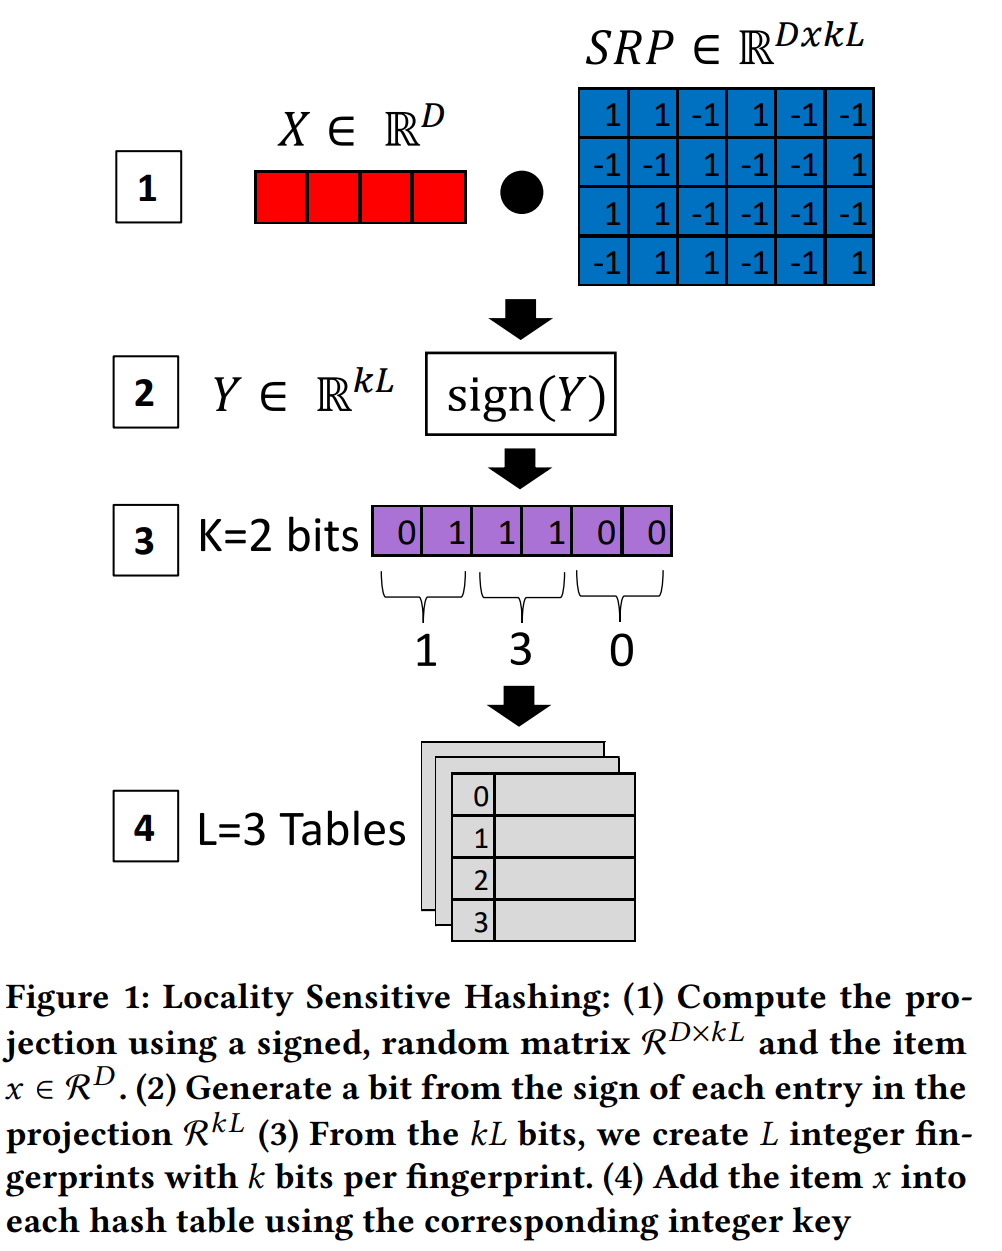
\includegraphics[width=0.5\textwidth]{images/lsh.png}
\end{frame}

\begin{frame}
    \frametitle{LSH query phase}
    \begin{itemize}
        \item Now, given a query $Q$, we first compute the $K$ hashes for each table 
        \item Then we retrieve all the elements in the corresponding bucket of that table
        \item The union of all the elements from the $L$ buckets is the \structure{candidate set}
        \item for nearest-neighbour we then further filter the candidate set to get the possible answers
        \item $K$ reduces false positives and $L$ decreases false 
        negatives
        \item An item $x$ is in the candidate set with probability $1-(1-p^{K})^{L}$
        \item Here $p \propto \operatorname{Sim}(Q,x)$
    \end{itemize}
    

\end{frame}

\subsection{Sampling Approach to LSH}

\begin{frame}
    \frametitle{Hashing-Based Sampling}
    \begin{itemize}
        \item Essentially LSH samples, in sub-linear time, elements with probability $1-(1-p^{K})^{L}$
        \item Therefore, we can use the candidate set returned by LSH as the result of an adaptive sampling algorithm
    \end{itemize}
    \begin{block}{Intuition}
        \begin{itemize}
            \item Consider a node $i$ with weight $w_{i}$ and an input $x$
            \item Activation is monotonic function of $w_{i}^{T}\cdot x$
            \item Finding the \structure{active neurons} is searching each $w_{i}$ and finding the ones with largest inner product
            \item Can do this efficiently using LSH and hash tables
        \end{itemize}
    \end{block}
\end{frame}

\begin{frame}
    \frametitle{Intuition}
    \centering
    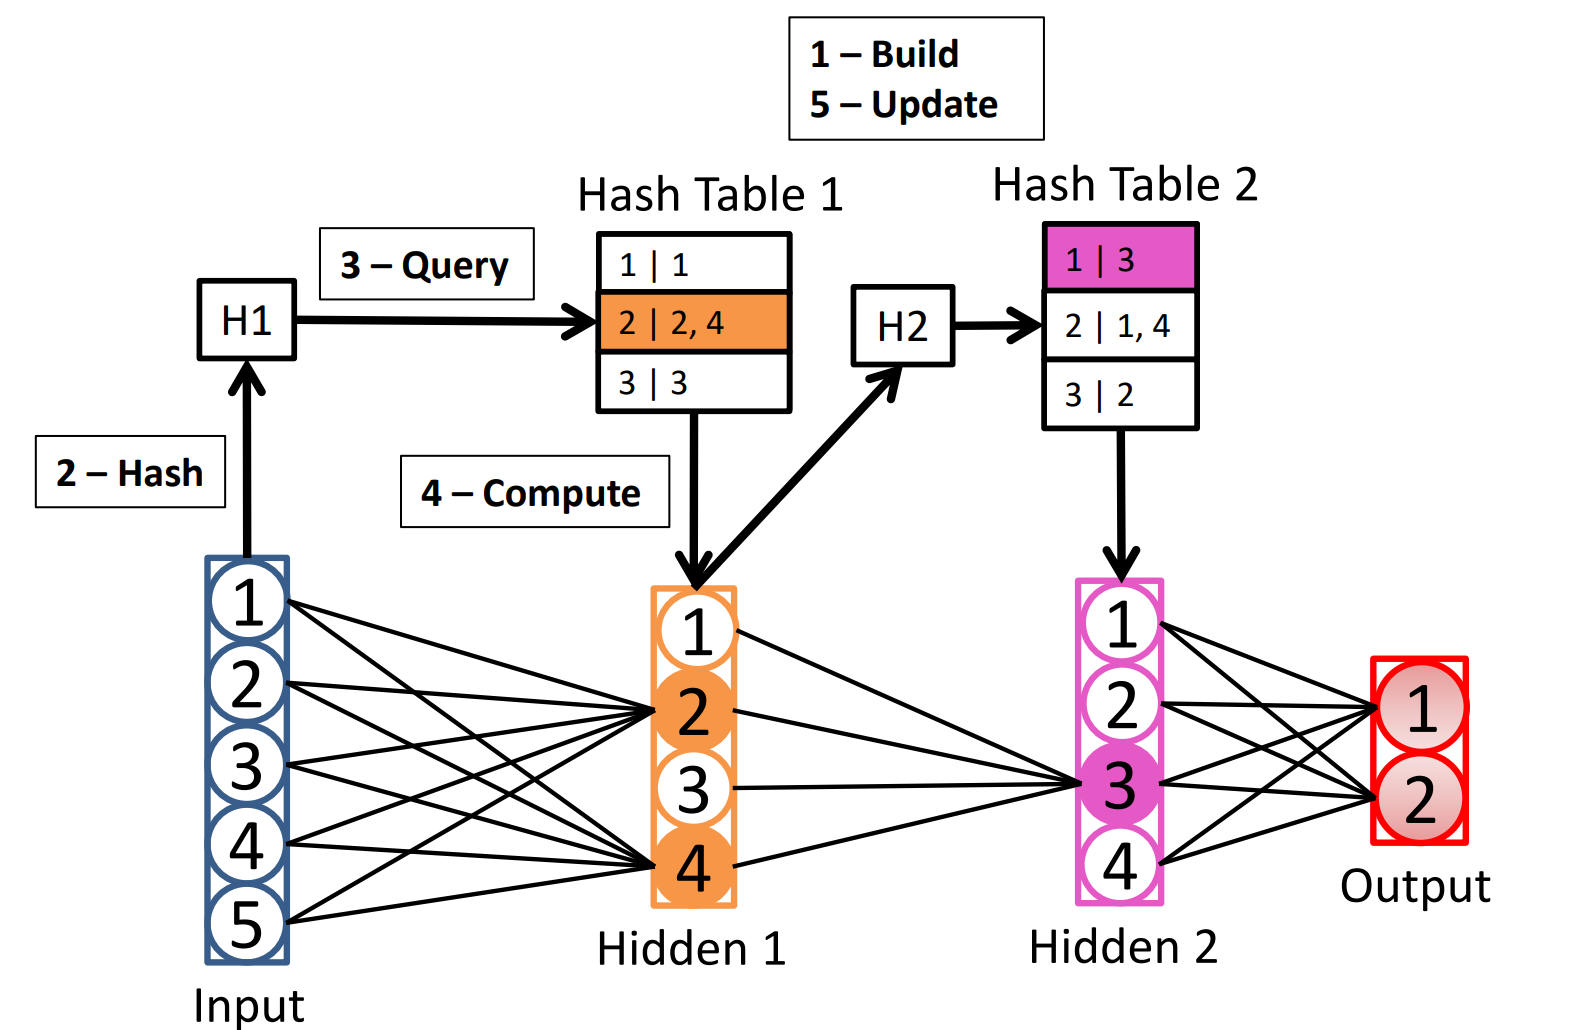
\includegraphics[width=\textwidth]{images/intuition.png}
    

\end{frame}
\subsection{Additional LSH tricks}
\begin{frame}
    \frametitle{LSH tricks}
    \begin{enumerate}
        \item Hashing inner products 
        \begin{itemize}
            \item Maximum Inner Product Search (MIPS): $p = \argmax_{x\in \mathcal{S}}q^{T}x$
            \item Nearest neighbour search (NNS): $p=\argmin_{x\in \mathcal{S}}\|q-x\|_{2}^{2}$
            \item Equivalent if norm of every element $x\in \mathcal{S}$ is constant. This is not the case for neural network weights.
            \item In regular LSH, $\operatorname{Pr}[h(x)=h(x)]=1$ is closest neighbour for query $x$
            \item \cite{shrivastava2014asymmetric} proposes using an asymmetric transformation to solve MIPS using LSH
        \end{itemize}
        \item Large $L$ for good estimates in vanilla LSH
        \begin{itemize}
            \item \cite{lv2007multi} proposes Multi-probe LSH which  reduces number of tables
            \item When querying, probe nearby buckets as well
            \item Do this by flipping a few bits in the hash for that table 
        \end{itemize}
    \end{enumerate}
\end{frame}

\section{Implementation}

\begin{frame}
    \frametitle{LSH Implementation}

    \centering
    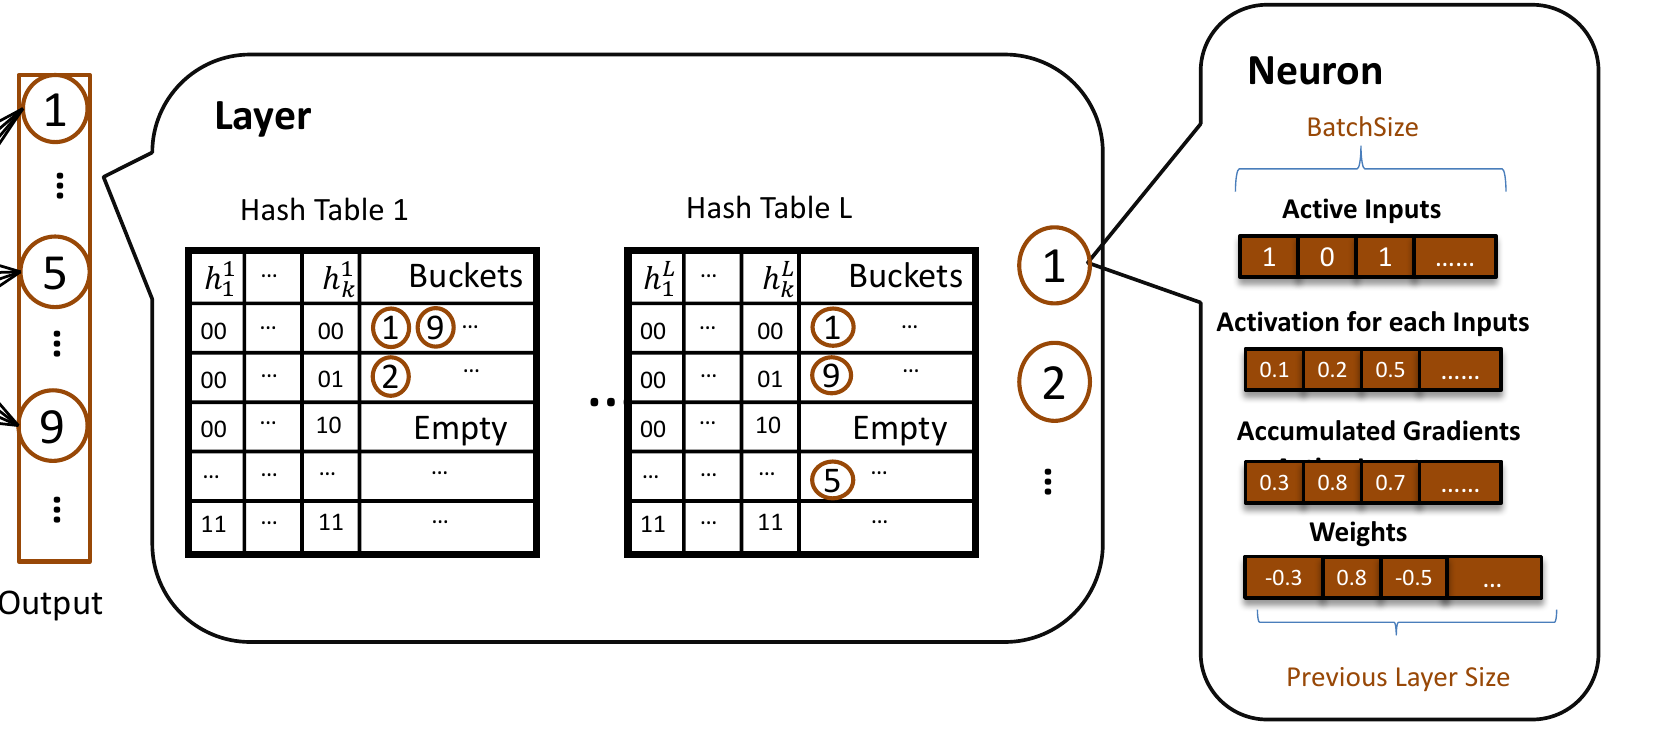
\includegraphics[width=\textwidth]{images/SLIDE.png}
    

\end{frame}

\begin{frame}
    \frametitle{Overview of Implementation}
    \begin{itemize}
        \item Each batch is \structure{processed in parallel} using simple OpenMP
        \item Only active neurons take part in forward and backpropagation
        \item The \structure{output softmax} is also computed only on active neurons
        \item After gradients are updates the hash tables are updated
        \item Can use Simhash or Densified Winner Take All (DWTA) hash families
    \end{itemize}

\end{frame}

\begin{frame}
    \frametitle{Benefits}
    \begin{itemize}
        \item Highly sparse active set, as small 5\% of all neurons
        \item Each update is computationally efficient
        \item Gradient updates are sparse $\rightarrow$ parallel ASGD
        \item Can choose different sampling  
    \end{itemize}
    

\end{frame}
\section{Results}

\begin{frame}
    \frametitle{Results}
    SWITCH TO OTHER SLIDES
    

\end{frame}
\begin{frame}
    \frametitle{}

    \centering \Large
    \emph{Questions or Comments}

\end{frame}

\bibliography{sources}
\bibliographystyle{apalike}
\end{document}